\chapter{Практические результаты}
\section{Наибольшая общая Абелева подстрока}
\subsection{Случай бинарного алфавита}

Первое, что хочется сделать~--- посмотреть, как же ведет себя на практике матожидание наибольшей общей Абелевой подстроки двух случайных бинарных строк. 

Я выполнил на своем ноутбуке (на кластере канеш) $10^4$ запусков поиска НОАП для различных $n$ до $10^4$. Такого количества запусков оказалось достаточно, чтобы среднее значение примерно сошлось (мб даже стоит попруфать, дисперсию там какую-нить оценить). Полученный результат можно увидеть на рисунке 1.

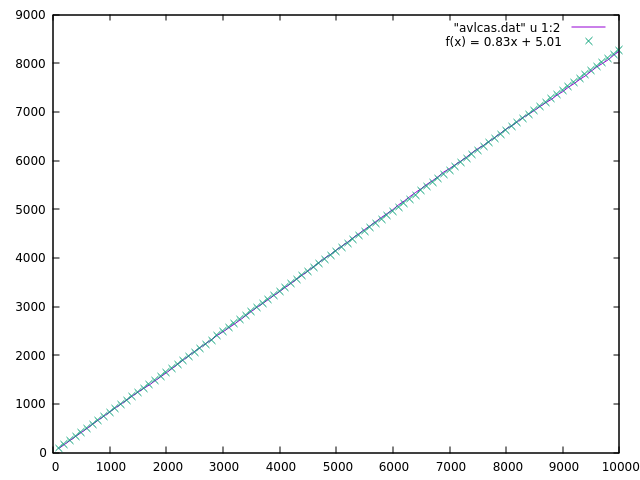
\includegraphics{pics/avlcas.png}
%TODO пронумеровать графики

Видно, что функция ведет себя очень точно как прямая $y=0.83x$, что подтверждает линейные оценки как сверху, так и снизу.

Вычислить точное значение этого коэффициента, или строгие оценки на него сверху и снизу остается открытой задачей. 

%\subsection{Общий случай}
%Пусто? Ну я канеш могу закодить то что я придумал но не оч хочется(((

\section{Количество Абелевых подквадратов}

Реализованный алгоритм решения $3SUM^+$ был протестирован на строке из одинаковых символов, и на наборе пар случайных бинарных строк. На практике он показал себя достаточно плохо, во много раз проигрывая наивному решению за $\mathcal{O}(n^2)$.

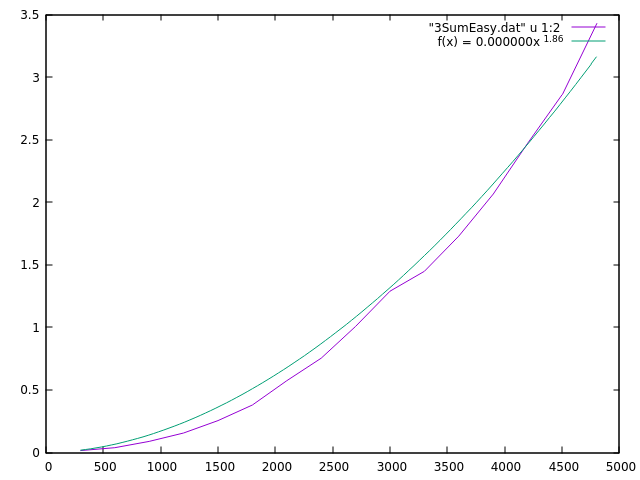
\includegraphics[scale=1]{pics/4.png}
%TODO пронумеровать графики

На этом графике можно увидеть зависимость времени работы решения в секундах от $n$~--- длины строк, данных на вход, на тесте со строками из одинаковых символов. График действительно довольно похож на $n^{1.86}$, но из-за нескольких логарифмов в асимптотике растет несколько быстрее. 

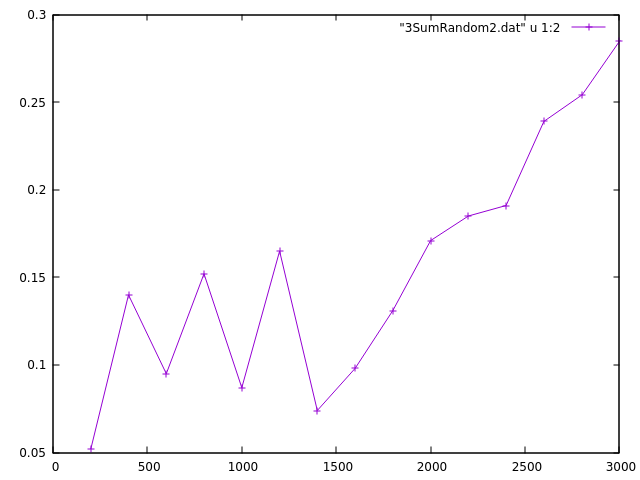
\includegraphics[scale=1]{pics/5.png}
%TODO пронумеровать графики

На этом графике можно увидеть зависимость времени работы решения в секундах от $n$~--- длины строк, данных на вход, на тесте со случайными строками из двух различных символов.

Время работы алгоритма довольно сильно меняется как от запуска к запуску из-за разных тестов, так и от различных значений $n$, так как различные ветки программы выполняются с разными вероятностями и работают разное время~--- не приходится удивляться некоторому увеличению производительности при увеличении $n$.
